\documentclass[12pt, oneside, a4paper]{article}

\usepackage[utf8]{inputenc}     % kodowanie na UTF-8
\usepackage[polish]{babel}
\usepackage{csquotes}
\usepackage[
    style=alphabetic, % numeric, alphabetic, authoryear, 
    backend=biber,]{biblatex}
\addbibresource{bibliografia.bib}   % dołączenie pliku bibliografi 


\usepackage[T1]{fontenc}           % ,,europejski'' układ fontów (Cork)
%\usepackage[OT4,plmath]{polski}   % Zestaw czcionek
\usepackage{times}                 % Times - Czcionki wektorowe
\usepackage{graphicx}              % Wstawianie grafiki
\usepackage{geometry}              % 
\usepackage[usenames]{color}       % Palety kolorów zdefionwanych
\usepackage{fancyhdr}              %
%\usepackage{titlesec}              %
%\usepackage{tocloft}               %
\usepackage{amsmath}               % Moduł matematyczny AMS
\usepackage{amsfonts}              % pakiet czcionek AMS
\usepackage{amsthm}                % Definicje matematyczne AMS
\usepackage[dvipsnames,svgnames]{xcolor}    % Zestaw kolorów             
\usepackage{indentfirst}           % uzyskanie wcięcia przy pierwszym akapicie
\usepackage{nameref}               % pakiet referencji do pełnych nazw rozdziałów
\usepackage{subcaption}
\usepackage{array}
\usepackage{footnote}


\usepackage[dvipsnames,svgnames]{xcolor}
  % zdefiniowane kolory dla formatowania linków, bibliografi oraz spisu treści
  \definecolor{wine}{RGB}{149,56,56}
  \definecolor{wine-stain}{RGB}{200,125,125}
  \definecolor{grass-green}{RGB}{53,161,103}
  \definecolor{ocean-blue}{RGB}{9,63,97}


\usepackage{indentfirst}   % uzyskanie wcięcia przy pierwszym akapicie
\usepackage[
  font=small,
  format=hang,
  labelformat=simple,
  justification=justified,
  labelsep=colon]{caption}       % pakiet dla podpisów np: dla lstlintings
\usepackage{nameref}       % pakiet referencji do pełnych nazw rozdziałów
\usepackage{enumerate}
\usepackage{multirow}      % pakiet dla łaczenia wierszy w tabelach
\usepackage[framemethod=tikz]{mdframed}     % pakiet zastępujący mało modalny \fbox
\usepackage{listings}      % pakiet dla kodów zródłowych


%------------------------------------------------------------------

% Dodanie komendy dla caption + source
\newcommand*{\captionsource}[2]{%
  \caption[{#1}]{%
    #1%
    \\\hspace{\linewidth}%
    {Źródło:} #2%
  }%
}

% Wydruk kodu latexa w ramce
\newmdenv[
    skipabove=0.2cm,
    skipbelow=0,
    nobreak=true]{outputbox}

%------------------------------------------------------------------

\lstloadlanguages{TeX}
\lstset{
  literate={ą}{{\k{a}}}1
           {ć}{{\'c}}1
           {ę}{{\k{e}}}1
           {ó}{{\'o}}1
           {ń}{{\'n}}1
           {ł}{{\l{}}}1
           {ś}{{\'s}}1
           {ź}{{\'z}}1
           {ż}{{\.z}}1
           {Ą}{{\k{A}}}1
           {Ć}{{\'C}}1
           {Ę}{{\k{E}}}1
           {Ó}{{\'O}}1
           {Ń}{{\'N}}1
           {Ł}{{\L{}}}1
           {Ś}{{\'S}}1
           {Ź}{{\'Z}}1
           {Ż}{{\.Z}}1,
  language=bash,
  captionpos=t,
  tabsize=3,
  frame=lines,
  keywordstyle=\color{blue},
  commentstyle=\color{darkgreen},
  stringstyle=\color{red},
  numbers=left,
  numberstyle=\textnormal,
  numbersep=12pt,
  breaklines=true,
  showstringspaces=false,
  basicstyle=\ttfamily,
  emph={label}
}

%---------------------------------------------------------------------------

\theoremstyle{plain}
\newtheorem{thm}{Twierdzenie}[section]
\newtheorem{lem}[thm]{Lemma}
\newtheorem{prop}[thm]{Założenie}
\newtheorem*{cor}{Wniosek}

\theoremstyle{definition}
\newtheorem{defn}[thm]{Definicja}
\newtheorem{conj}{Przypuszczenie}[section]
\newtheorem{exmp}{Przykład}[section]

\theoremstyle{remark}
\newtheorem*{rem}{Remark}
\newtheorem*{note}{Note}

%---------------------------------------------------------------------------

% Ustawienie linkowania dokumetu oraz elementów wyświetlania pdfa (4.7.4 z latex w 129 minut)
\usepackage{hyperref}
\hypersetup{
  unicode=true,           % używać znaków z alfabetów niełacińskich zakładkach Acrobata
  pdftoolbar=true,        % show Acrobat’s toolbar?
  pdfmenubar=true,        % show Acrobat’s menu?
  pdffitwindow=false,     % window fit to page when opened
  pdfstartview={FitH},    % fits the width of the page to the window
  pdftitle={},                % title
  pdfauthor={Maciej Sypień},  % author
  pdfsubject={Subject},       % subject of the document
  pdfcreator={Maciej Sypień}, % creator of the document
  pdfproducer={Maciej Sypień},     % producer of the document
  pdfkeywords={keyword1} {key2} {key3}, % list of keywords
  pdfnewwindow=true,          % links in new window
  linktoc=page,                % Ustawienie linków dla bibliografi (none, all, page, section)
  colorlinks=true,            % false: boxed links; true: colored links
  linkcolor=wine,             % color of internal links (change box color with linkbordercolor)
  citecolor=grass-green,      % color of links to bibliography
  filecolor=magenta,          % color of file links
  urlcolor=ocean-blue,        % color of external links
}

%---------------------------------------------------------------------------
% Definicje własnych, nowych makr

% poniższe makra wymagają pakietu 'xcolor'
\newcommand{\red}[1]{{\color{RedOrange}{#1}}}
\newcommand{\yellow}[1]{{\color{Dandelion}{#1}}}
\newcommand{\green}[1]{{\color{LimeGreen}{#1}}}
\newcommand{\RED}[1]{{\colorbox{RedOrange}{#1}}}
\newcommand{\YELLOW}[1]{{\colorbox{Dandelion}{#1}}}
\newcommand{\GREEN}[1]{{\colorbox{LimeGreen}{#1}}}


% Lowercase \nameref = \lnameref
\newcommand{\lnameref}[1]{%
\bgroup
\let\nmu\MakeLowercase
\nameref{#1}\egroup}

% First UpperCase then lowercase = \fnameref
\newcommand{\fnameref}[1]{%
\bgroup
\def\nmu{\let\nmu\MakeLowercase}%
\nameref{#1}\egroup}

% helper for lowercase newcommands
\newcommand{\nmu}{}

%---------------------------------------------------------------------------

\title{
	\LARGE{Uniwersytet Ekonomiczny w Krakowie}\\
	\vspace{0,3cm}
	\Large{Wydział Zarządzania}\\
	\vspace{3cm}
	\Huge{Możliwości promocji w najpopularniejszych mediach społecznościowych}
	\vspace{2cm}
}
\author{Łukasz Suder\\ Maciej Sypień}
\date{\today}

%---------------------------------------------------------------------------

\begin{document}
\nocite{*}     % wszystkie pozycje z bibliografii

\maketitle     % tworzy tytuł + imiona autorów + datę

\begin{abstract}
Dokument ten prezentuje możliwości działań promocyjnych firm w~najpopularniejszych mediach społecznościowych.\\
Praca została przygotowana w systemie składowania tekstu \LaTeXe .
\end{abstract}

\clearpage
\tableofcontents     % wstawia spis treści
\clearpage

%---------------------------------------------------------------------------

%----------------------------------------------------------------------------------------
%	Wprowadzenie
%----------------------------------------------------------------------------------------

\section{Wprowadzenie}
\label{sec:wprowadzenie}

Tu znajdzie się wstęp do naszego dokumentu.

\begin{defn}[Serwis społecznościowy]
bla bla bla definicja
\end{defn}

%-------------------------------------------------------------------------

\clearpage

\section{Facebook}
\label{sec:facebook}
Tu najdzie się duuszoo informacji o fejsie dostarczonych przez Ciebie Łukaszu :).


%------------------------------------------------------------------------
\clearpage

\section{Google+}
\label{sec:google-plus}
Google+ znany również pod innymi nazwami takimi jak \emph{Google Plus} lub \emph{G+}, to serwis społecznościowy będący własnością firmy Google Inc.

Serwis ten podobnie jak Facebook, umożliwia dzielenie się informacjami między użytkownikami sieci poprzez możliwość zamieszczania tekstów, zdjęć, wideoklipów czy linków do innych zasobów w sieci, promując je własną marką lub nazwiskiem.

W sieci krąży bardzo wiele różnych wersji logotypu Google+ czy g+, które są często zmieniane i komponowane specjalnie pod kolorystykę i układ skórek witryn internetowych, jednak aby sprecyzować rzeczywisty wygląd logotypów przedstawiono na rysunku \ref{fig:logo-google} dwa rodzaje logotypów występujące oficjalnie na stronie Google+ (\url{https://plus.google.com/}).

\begin{figure}[!h]
\centering
\begin{subfigure}{.5\textwidth}
  \centering
  
\includegraphics[width=.4\linewidth]{images/googleplus_color.png}
  \caption{Logo tekstowe}
  \label{fig:sub1}
\end{subfigure}%
\begin{subfigure}{.5\textwidth}
  \centering
  \scalebox{0.7}
  {
      
\includegraphics[width=.4\linewidth]{images/google-plus-logo.png}
  }  
  \caption{Logo graficzne}
  \label{fig:sub2}
\end{subfigure}
\captionsource{Rodzaje logotypów występujących na witrynie Google+}{\url{https://plus.google.com/}}
\label{fig:logo-google}
\end{figure}

Spośród wszystkich portali społecznościowych Google+ odróżnia się od konkurencji tym, że pragnie stawiać na wiarygodność informacji dostarczanej od użytkowników\footnote{W myśl założeń firmy Google, użytkownika portalu reprezentuje jakaś rzeczywista osoba lub organizacja, przez co uwiarygadnia dany podmiot. Osoby lub firmy nie będące fikcyjnym tworem przesyłając informacje, opinię, uwagę, ect. wnoszą pozytywny wkład w ogólny przekaz informacji, a nie sztuczną bańkę informacyjną ,,produkowaną i przekazywaną dalej'' w sieć, jako zabieg marketingowy do szybszego i skuteczniejszego wpływania na działania użytkowników.} oraz lokalność.

Umieszczenie informacji, zdjęć, nagrań wideo nie są jedynymi działaniami jakie oferuje g+. Portal pozwala także na tworzenie wydarzeń, opiniowanie produktów czy usług oferowanych przez firmy promujące się w społeczności poprzez rozdawanie plusików, a także integralny dostęp do innych usług oferowanych przez firmę Google zwiększając tym samym ofertę przystąpienia do społeczności.

%-----------------------------------------

\subsection{Promocja firmy, a Google+}
W chwili obecnej tj. 2 kwartale 2014 roku wyszukiwarka Google zajmuję 1 miejsce wśród narzędzi do wyszukiwania informacji w Polsce (95,59\% udziału rynku), zaraz za nią MSN (2,57\%) oraz Yahoo (0,97\%) \cite{url:gemius-ranking-silnikow-wyszukiwarek}.

Google będąc największym potentatem rozwiązań wyszukiwania informacji w internecie na polskim rynku można pokusić się nawet o stwierdzenie że jest niemal monopolistą rynkowym, spychając rywali na wąski margines.

Tak ogromny udział w rynku zapewnia niemal nieograniczone możliwości kreacji promocji w sieci. Jednak z punktu widzenia wolności i konkurencyjności rynku, ,,wyszukiwarek'' baron dyktuje koszty promocji wszystkim tym, którzy korzystają z jego produktów --- a jest to niemal całość polskiego społeczeństwa $\sim$96\%. Tak wielki procent udziałów w rynku, poniekąd zmusza firmy do skorzystania z oferty Google, jeśli chcą dotrzeć do wiekszości polskich internatów. \\


Jednym z darmowych narzędzi ułatwiających promocję firmy wśród mediów społecznościowych jest wcześniej wspomniany google+. Google+ jako jedna z usług dostarczanych przez firmę Google ma za zadanie łączyć społeczność portalu i personalizować ich użytkowników, a przez to uwiarygadniać oraz dzielić się treściami pochodzącymi z wiarygodnego, zaufanego źródła --- przykładowo naszego przyjaciela Pana Michała, który istnieje (nie jest fikcyjną wykreowaną przez media/marketing postacią) i wyraził swoją opinię o jednym z przedmiotów promowanych przez firmę. Dzięki sieci Google+ wiem z dużym prawdopodobieństwem, że opinia Pana Michała jest wiarygodna, ponieważ go znam (widuję na co dzień), a dzięki dobrej opinii o wykonaniu usługi istnieje również większa szansa, że i ja skorzystam z usługi.\\

Ta krótka, lecz ważna notka z punktu widzenia osoby prawnej, w wąskim stopniu przybliża działanie idei portalu oraz istotności potrzeby promocji w nim (a także wszystkich usługach oferowanych przez Google, które poniekąd tworzą jedną spójną całość uzupełniając się wzajemnie). 

Rozmawiając o usłudze Google+ dyskutujemy tak na prawdę o narzędziu spajającym ze sobą pozostałe usługi dostarczane przez firmę Google w postaci jednego, ułatwiającego zarządzanie Panelu Google+.

%-------------------------------------------

\subsection{Panel Google+}
Panel Google+ to obszar skupiający w jednym miejscu kluczowe informacje dotyczące różnych obszarów istotnych w prowadzeniu firmy w internecie (tu celowo pomijam użytkownika indywidualnego, ponieważ nie jest on tematem dysputy w niniejszej publikacji).\\




\begin{figure}[!h]
\centering
    \scalebox{0.21}
    {
        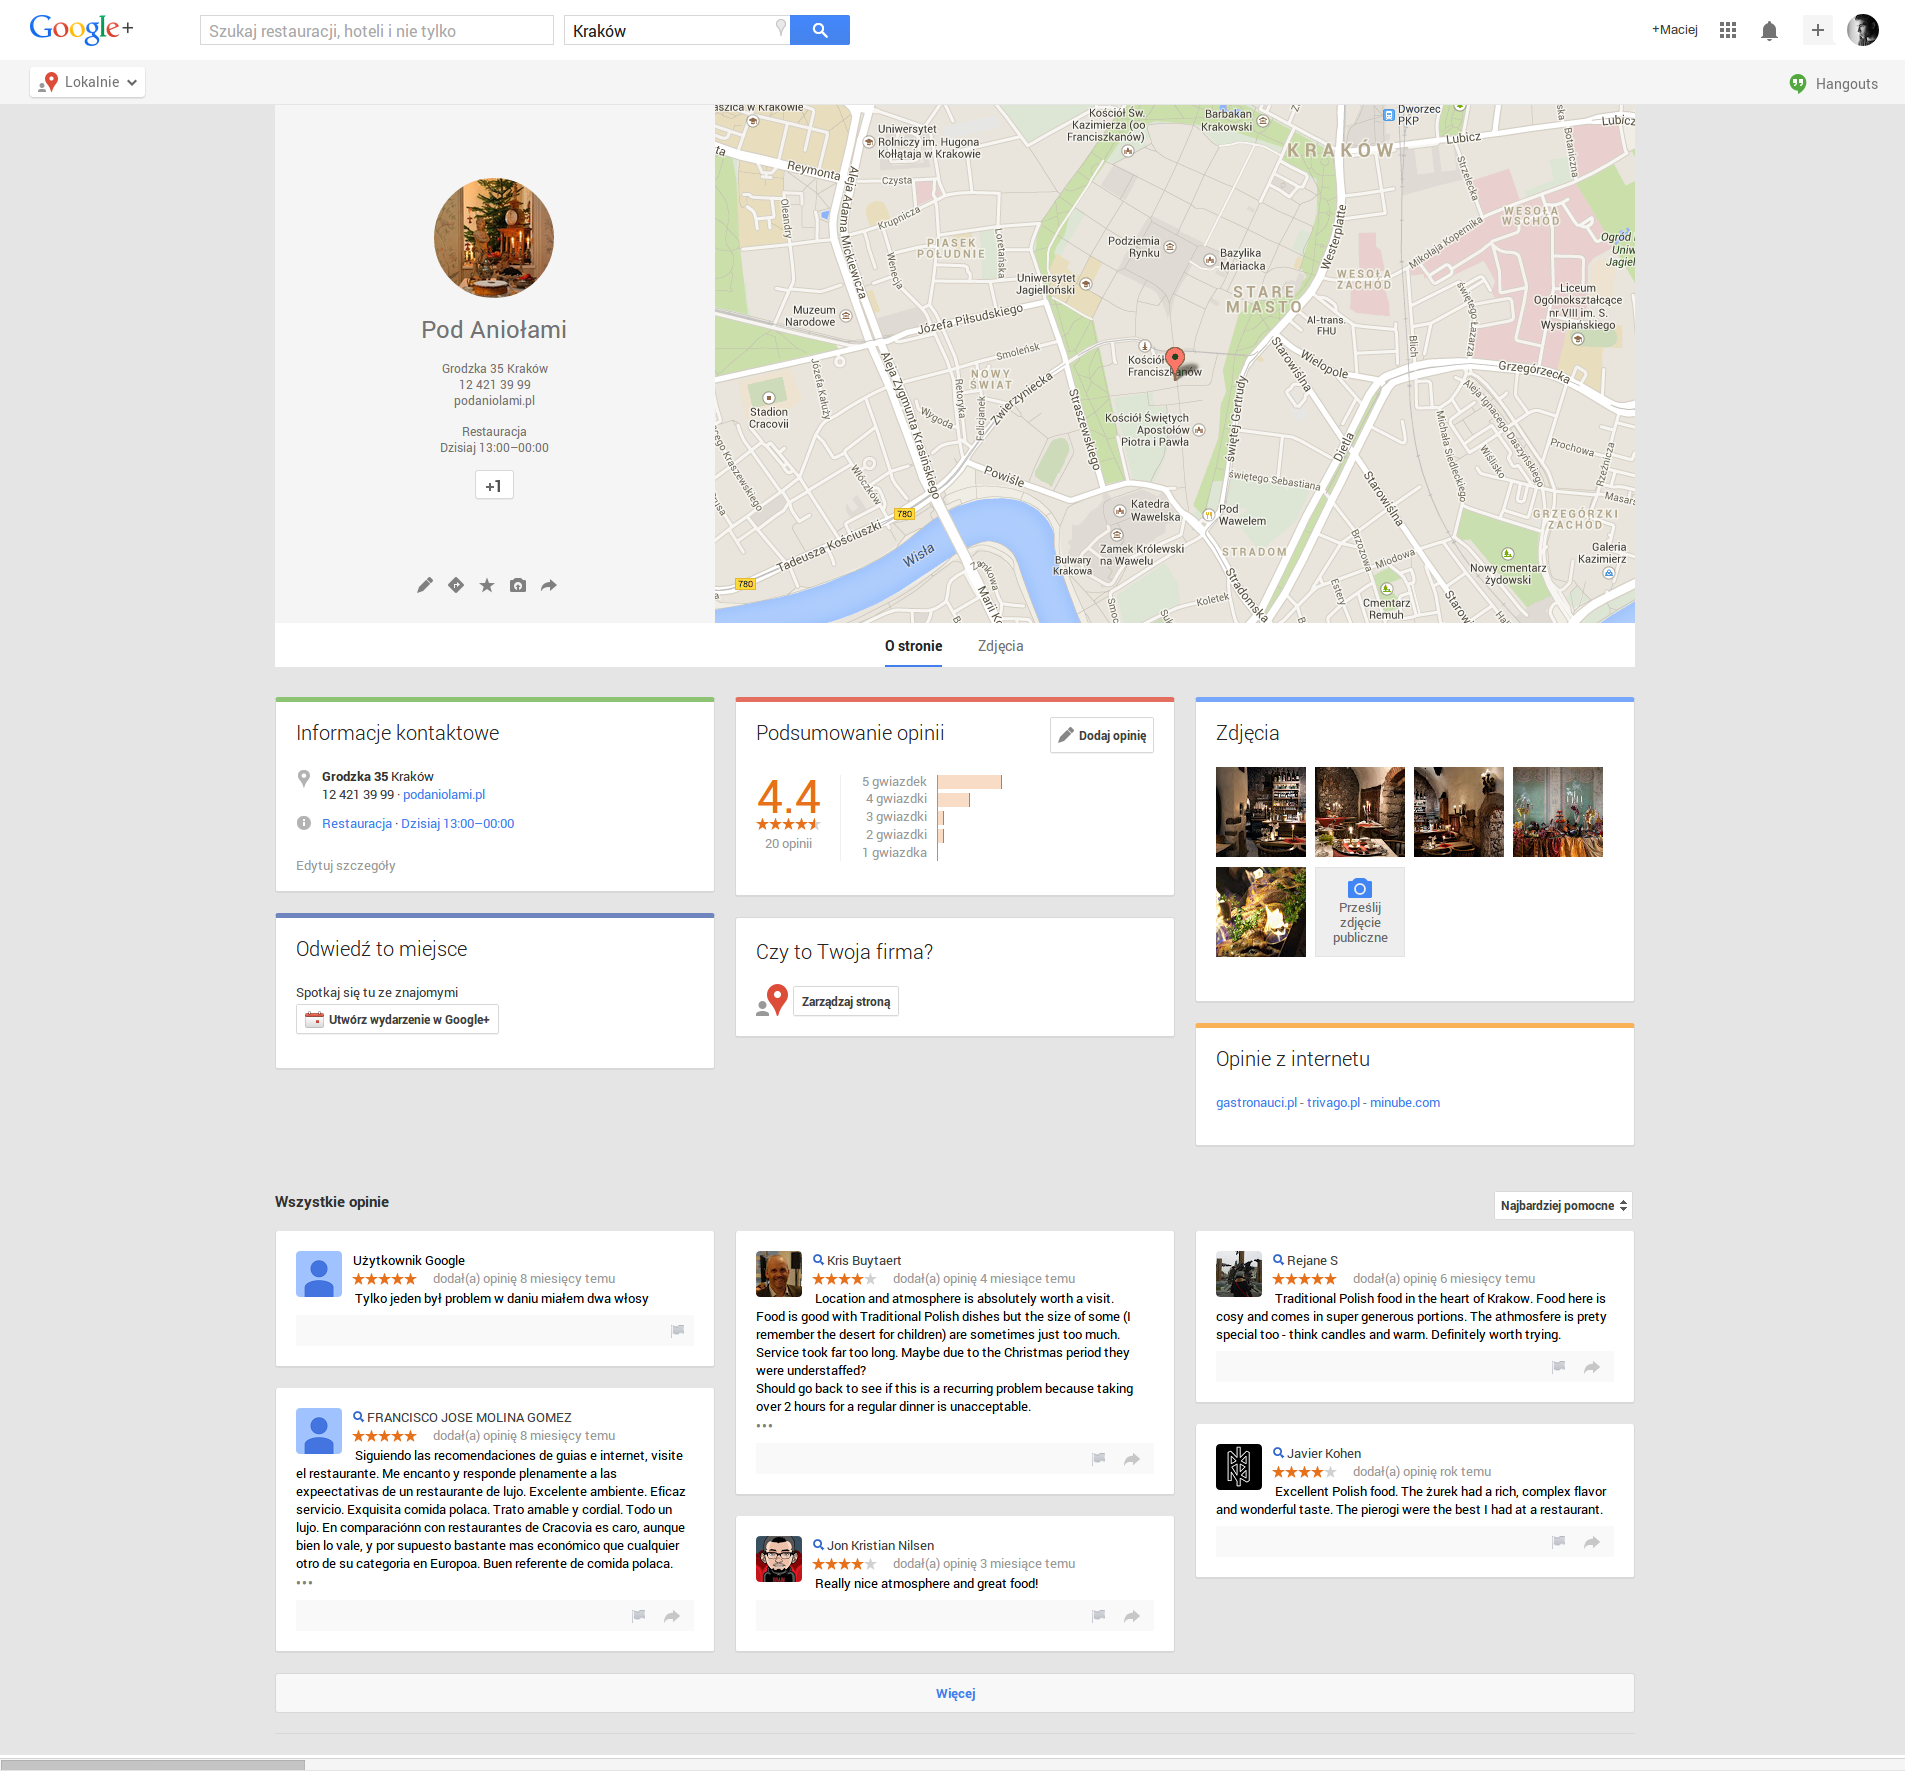
\includegraphics{images/pod-aniolami-google-plus.png}
    }
    \captionsource{Przykładowy profil firmy w Google+}{Opracowanie własne}
    \label{fig:sample-google-plus-company-profile-page}
\end{figure}


Panel Google+ dostarcza m.in:

\begin{itemize}
\item Możliwość aktualizacji danych firmy w 1 miejscu;

\item Narzędzia sprawdzające kompletność i zgodność witryny z wyszukiwarką \mbox{Google};

\item Wyświetlać wpisy innych użytkowników oraz tworzyć własne z informacjami, zdjęciami i filmami.

\item Szeroka interakcja z klientami poprzez budowanie precyzyjnego grona odbiorców oraz udoskonalanie swoich zasobów odpowiadając na opinie użytkowników o firmie/usłudze.

\item Rozmawiać bezpośrednio ,,twarzą w twarz'' z klientami dzięki usłudze Google Hangouts (internetowy odpowiednik Skype lub Viber);

\item Przeglądać szeroki zakres różnego typu statystyk dotyczących firmy a w tym:
    \begin{itemize}
    \item Najpopularniejsze wyszukiwania na temat firmy w wyszukiwarce Google;
    \item Skąd klienci wyznaczą trasy dojazdu do placówki dzięki usłudze Google Maps;
    \item Sprawdzenie popularności firmy wśród społeczności Google+;
    \end{itemize}

\item Zarządzać reklamami, w tym także poprzez integrację z usługą AdWords Express;

\item Mobilność dostarczanych rozwiązań (Smartphone, Tablet, Komputer);
\end{itemize}

%----------------------------------------------------------------------

\subsection{Możliwości promocji w Google+}
\
Model promocji działalności w Google+ jest dość jasny --- tworząc własny profil lub inaczej stronę (ang. \textit{wall}) umieszczamy wszystkie rzeczy dotyczące firmy tj. informacje oraz mapę dojazdu do firmy, tworzymy posty z atrakcyjnymi ofertami usługami lub produktów, a w zamian uzyskujemy ogromne i w miarę możliwości wiarygodne\footnote{Wiarygodność jest tu ujęta w cudzysłów, ze względu na fakt, iż prawdopodobnie nigdy nie osiągnie poziomu 100\%. Zawsze jakiś odsetek opinii czy uwag na temat produktu będzie przejaskrawiony w negatywną stronę lub po prostu zrobiony z premedytacją (w ramach zagrań nieczystej konkurencji).\\ Jednak ogólne założenia wiarygodności użytkowników w systemie Google+ pozwalają nam z dużym prawdopodobieństwem twierdzić, że opinia danego klienta jest jak najbardziej prawdziwa i wartościowa, tak więc rozsądnie jest brać je wszystkie pod uwagę.} miejsce zwrotów opinii wśród użytkowników, który skorzystali z naszych usług. 

\noindent Dodatkowo dzięki informacji zwrotnej od klientów (posiadających konto Google+) możemy szybko skorygować lub udoskonalić naszą ofertę, a tym samym promując ją dalej wśród znajomych naszych klientów, którzy właśnie skorzystali z części naszej oferty i wyrazili opinię. 

Jak widać na rysunku \ref{fig:sample-google-plus-company-profile-page} przedstawiającym schludny, stonowany, firmowy profil Google+ jednej z Krakowskich restauracji, który posłuży nam jedynie jako wstępny szablon informacji o modelach promowania się wraz z siecią google+.

To jednak tylko ogólny zarys wstępu do poszczególnych kanałów jakie oferuje Google+. W dalszej części omówimy bardziej szczegółowo poszczególne możliwości usługi w nieco szerszym zakresie, w tym profity jakie niosą ze sobą dla inwestora chcącego dowiedzieć się co uzyska (lub straci) dzięki takiemu profilowi.

\subsubsection{\nmu Wszystko w jednym miejscu}
\label{subsubsec:wszystko-w-jednym-miejscu}
Dla wielu rekinów biznesu ale i nie tylko pewne przysłowie: ,,jak coś jest  do wszystkiego, to jest do niczego'' jest bardzo realne i sprawdza się. Jednak w tym kontekście naszego podrozdziału \lnameref{subsubsec:wszystko-w-jednym-miejscu}, główna strona profilu\footnote{Nota bene profil Google+ inaczej widzi właściciel konta, ponieważ posiada możliwość edycji materiałów na profilu, a nieco odmiennie widzi go klient lub po prostu inny użytkownik portalu google+, który może zaobserwować zwartą kondensacje danych w postaci prostej przewijanej witryny (aktualnie popularny i obserwowalny w internecie model tworzenia witryn www nie wymagający za dużo ,,męczenia się i klikania'', a jedynie oczekuje od użytkownika przewijanie strony coraz niżej --- taki rozwój stron może być nawet traktowany jako kompensacja rozwoju internetu)}, czyli tak zwany \textit{wall} zawiera wszystkie najpotrzebniejsze informacje dla klienta co widać na rysunku \ref{fig:sample-google-plus-company-profile-page} i w tym kontekscie powinna być rozpatrywana. Nie jako narzędzie do wszystkiego, chodź za takie może uchodzić ponieważ jest elementem łączącym pozostałe usługi firmy Google przykładowo tj. Hangouts, Google Maps czy AdWords. 

\noindent Jednak oprócz spoiwa różnych usług, którym z pewnością jest google+, zapewnia również interakcję z użytkownikiem poprzez umieszczanie postów (w tym tekstu, obrazu, wideo) oraz wydawanie opinii klientów o swoich usługach. 

W głównej mierze ma być miejscem profesjonalnej i rzetelnej informacji dla klienta. Pytanie tylko czy stosunkowo niedawne wejście na rynek pozwoli poważnemu i profesjonalnemu Google+ wyprzeć bardziej frywolnego, kierowanego na luźniejsze relację giganta jakim jest Facebook\footnote{Firma Google posiada nieco odmienne założenia społecznościowe dla swoich produktów. Google stawia na wiarygodności i rzetelność opinii na których można polegać i równie dobrze szybko odnaleźć (dzięki lepszej współpracy z własną wyszukiwarką). To są niepodważalne cechy profesjonalizmu dla firm. 
Flagowy produkt firmy Facebook skupia się natomiast na nieco innych założeniach. Mianowicie relacjach międzyludzkich głęboko zakorzenionych w ludziach jak np.: związkach(słynny status ,,w związku''), przyjaźniach, dzieleniem się informacjami w bliskim kontakcie z przyjaciółmi. Model produktu Facebook moim zdaniem ma zastosowanie dla nieco odmiennej grupy firm, niż bardziej uniwersalny Google+, co nie oznacza że zamyka im drogę. Jednak nie wszystko co związane z firmą, w oficjalny sposób można wrzucić na Facebook z racji różnego modelu świadczonych usług obydwu produktów.}.

%--------------------------

\subsubsection{Ucz się, dziel się i odkrywaj}
\red{
, a raczej jako miejsce gdzie możemy znaleźć wszystko co potrzebne w jednym miejscu. Możemy zaobserwować tam unifikację wyglądu profilu, a inaczej mówiąc ujednolicenie stylizacji strony celem lepszej orientacji klienta aby ,,nie zgubił się'', gdy przypuszczalnie będzie odwiedzać kilka lub kilkanaście różnych profilów różnych firm.

Idealnie można na nim wyróżnić adres oraz mapę dojazdu do firmy.

Zaletą wizualną ale także funkcjonalną dla klienta jest unifikacja. Większość profili można zmienić ale w jeden podobny do siebie sposób
}

\subsubsection{Budowanie społeczności}
Wielokrotnie wspominany profil w Google+ w dostarcza wielu różnych usług pomagających w relacjach społecznościowych.

Jedną z nich są Kręgi (ang. Circles). To usługa pozwalająca budować grupy kontaktów i tym samym tworzyć łatwe połączenia biznesowe zanim będziemy próbować sprzedać swój produkt dalej. To ważne dla wielu osób (z punktu widzenia psychologicznego również) z tego względu, że tworzy ,,wrażenie znajomości'' mimo iż np.: w rzeczywistości nie miała ona miejsca. Wtedy łatwiej o nawiązanie kontaktu, a jeśli ktoś ma go z swoich kontaktach i spodoba się to efekt domina rozprzestrzenia się samoistnie --- to bardzo prosta i przydatna rzecz podczas promocji własnej firmy dalej w świat.



\subsubsection{Słuchaj oraz wypowiadaj się}

\begin{itemize}
\item Opinie;
\item Hangouts;
\end{itemize}

%----------------------------------------------------------------------------------------
\clearpage
\section{Podsumowanie}

Każdy z portali społecznościowych wyraża nieco odmienne przewodnie idee. 


%---------------------------------------------------------------------------
%\clearpage

\printbibliography

\end{document}

\end{document}